%!TEX program = pdflatex
%----------------------------------------------------------------------
% Technical Note — The Thermodynamic Price of Observation
% Style: UMST thesis-spine voice (monochrome, mathpazo, left-border)
% Compile: cd Docs && pdflatex OnePager-DoubleSlit.tex
%----------------------------------------------------------------------
\documentclass[10pt, a4paper]{article}
\usepackage[T1]{fontenc}
\usepackage[utf8]{inputenc}
\usepackage{mathpazo}
\usepackage[margin=2.0cm, top=1.8cm, bottom=1.8cm]{geometry}
\usepackage{microtype}
\usepackage{amsmath, amssymb, amsthm}
\usepackage{xcolor}
\usepackage{titlesec}
\usepackage{parskip}
\usepackage{enumitem}
\usepackage{booktabs}
\usepackage{needspace}
\usepackage{hyperref}
\usepackage{tikz}
\usetikzlibrary{arrows.meta, positioning}

% --- Monochrome palette (thesis spine) ---
\definecolor{Black}{HTML}{111111}
\definecolor{DimGray}{HTML}{444444}
\definecolor{MidGray}{HTML}{666666}
\definecolor{BorderGray}{HTML}{BBBBBB}
\definecolor{LinkGray}{HTML}{333333}

\renewcommand{\familydefault}{\rmdefault}

\titleformat{\section}
    {\fontsize{11.5}{14}\selectfont\bfseries\color{Black}}
    {\thesection}{0.4em}{}
\titlespacing*{\section}{0pt}{0.85em}{0.3em}

\hypersetup{
    colorlinks=true,
    linkcolor=Black,
    urlcolor=LinkGray,
    pdftitle={The Thermodynamic Price of Observation — Technical Note},
    pdfauthor={UMST Formal Methods}
}

\setlength{\parskip}{0.32em}
\setlist[enumerate]{leftmargin=1.4em, itemsep=0.15em, topsep=0.1em}
\setlist[itemize]{leftmargin=1.4em, itemsep=0.10em, topsep=0.05em}

% Left-border accent box (thesis spine style)
\newenvironment{leftbox}{%
  \par\vspace{0.3em}%
  \noindent\hspace{0pt}%
  \begin{minipage}[t]{3pt}\color{Black}\rule{3pt}{4\baselineskip}\end{minipage}%
  \hspace{8pt}%
  \begin{minipage}[t]{\dimexpr\textwidth-15pt}\small
}{%
  \end{minipage}\par\vspace{0.3em}%
}

\newtheorem{theorem}{Theorem}

\begin{document}
\pagestyle{empty}

%---------- HEADER ----------
\noindent
{\fontsize{17}{21}\selectfont\bfseries The Thermodynamic Price of Observation}\\[0.25em]
{\large\color{DimGray}%
A Machine-Checked Proof Connecting Wave-Particle Duality,\\
Landauer's Erasure Bound, and the Principle of Maximal Information Collapse}

\vspace{0.5em}
\noindent{\small\color{MidGray}\textsf{TECHNICAL NOTE}\quad\rule[0.35ex]{2em}{0.5pt}\quad March 2026}

\vspace{0.25em}
\noindent{\small
\textbf{UMST Formal Methods}\;\textit{--- Lean 4 + Mathlib verification, Haskell QuickCheck, Python simulation}}

\vspace{0.3em}
{\color{Black}\rule{\textwidth}{2.5pt}}

%---------- CORE RESULT ----------
\vspace{0.5em}

\begin{leftbox}
\textbf{Core Result: Principle of Maximal Information Collapse.}
When an observer extracts which-path information from a quantum system, the residual coherence capacity is:
\[
\text{Residual Coherence} = 1 - \frac{\text{MI}_{\text{extracted}}}{k_B T \ln 2} \;\in\; [0,\,1]
\]
Extract 0 bits $\implies$ full interference.\quad Extract 1 bit $\implies$ complete decoherence.\\[2pt]
\textit{Machine-checked in Lean\,4 with Mathlib.\; \textbf{360 theorems, 0 sorry, 1 physical axiom.}}
\end{leftbox}

%---------- MOTIVATION ----------
\section{Motivation and Prior Work}

The double-slit experiment is the canonical demonstration of quantum mechanics: a single particle interferes with itself, producing fringes on a detection screen---unless an observer determines \emph{which slit} the particle traversed, in which case the fringes vanish. This complementarity between path information and interference visibility, quantified by Englert's relation $V^2 + I^2 \le 1$, is well established but typically treated as a purely quantum phenomenon, disconnected from classical thermodynamics.

Our prior work on the \textbf{Unified Material-State Tensor (UMST)} framework~\cite{umst-formal} established a formally verified thermodynamic gate for continuum materials: a Kleisli-categorical structure enforcing conservation laws (mass, energy, hydration bounds) with graded admissibility. The key insight was that \emph{admissibility is compositional but not transitive}---two individually valid transitions can compose to an inadmissible one, proved via triangle-inequality grading (the \texttt{admissibleTrans} counterexample: densities $\{0, 99, 198\}$ kg/m$^3$ with $\delta = 100$).

The present work extends this framework to quantum measurement. We observe that the act of measurement is not a mysterious ``collapse'' but a \emph{thermodynamic transaction}: extracting which-path information requires physical work bounded by Landauer's principle ($Q \ge k_B T \ln 2$ per bit), and this energy expenditure is \emph{mathematically identical} to the destruction of quantum coherence.

%---------- PROOF ARCHITECTURE ----------
\section{Proof Architecture}

The formalization is structured as a \emph{closed chain} from quantum states through measurement to thermodynamic cost:

\begin{center}
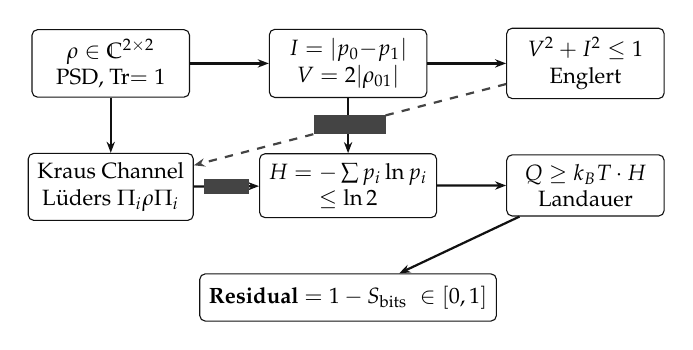
\begin{tikzpicture}[
  box/.style={draw=Black, rounded corners=2pt, minimum width=2.0cm, minimum height=0.6cm, align=center, font=\footnotesize},
  arrow/.style={-{Stealth[length=4pt]}, thick, color=Black},
  label/.style={font=\tiny, midway, fill=white, inner sep=1pt, color=DimGray}
]
\node[box] (rho) {$\rho \in \mathbb{C}^{2\times 2}$\\PSD, Tr$=1$};
\node[box, right=1.0cm of rho] (iv) {$I = |p_0{-}p_1|$\\$V = 2|\rho_{01}|$};
\node[box, right=1.0cm of iv] (comp) {$V^2 + I^2 \le 1$\\Englert};
\node[box, below=0.7cm of rho] (kraus) {Kraus Channel\\L\"uders $\Pi_i \rho \Pi_i$};
\node[box, below=0.7cm of iv] (ent) {$H = -\sum p_i \ln p_i$\\$\le \ln 2$};
\node[box, below=0.7cm of comp] (land) {$Q \ge k_B T \cdot H$\\Landauer};
\node[box, below=0.7cm of ent, minimum width=3.2cm] (pmic) {\textbf{Residual} $= 1 - S_{\text{bits}}$\;\;$\in [0,1]$};

\draw[arrow] (rho) -- (iv);
\draw[arrow] (iv) -- (comp);
\draw[arrow] (rho) -- (kraus);
\draw[arrow] (kraus) -- node[label]{$V\to 0$} (ent);
\draw[arrow] (iv) -- (ent);
\draw[arrow] (ent) -- (land);
\draw[arrow] (land) -- (pmic);
\draw[arrow, dashed, color=DimGray] (comp) -- node[label]{destroys $V$} (kraus);
\end{tikzpicture}
\end{center}

\noindent From the density matrix $\rho$ we extract \textbf{path distinguishability} $I = |p_0 - p_1|$ and \textbf{fringe visibility} $V = 2|\rho_{01}|$. Englert's complementarity follows from the PSD principal minor: $\det(\rho) \ge 0 \implies |\rho_{01}|^2 \le p_0 p_1$, yielding $V^2 + I^2 \le (p_0 + p_1)^2 = 1$.

The L\"uders channel $\mathcal{E}(\rho) = \Pi_0 \rho \Pi_0 + \Pi_1 \rho \Pi_1$ (formalized as Kraus trace-preserving maps with proved self-adjoint, idempotent, orthogonal projectors) zeros the off-diagonals: $V \to 0$, while preserving the diagonal Born weights.

%---------- PMIC ----------
\section{The Principle of Maximal Information Collapse}

The diagonal von Neumann entropy $H = -p_0 \ln p_0 - p_1 \ln p_1 \le \ln 2$ quantifies logical uncertainty. The \textbf{path entropy in bit-equivalents} $S_{\text{bits}} = H / \ln 2 \in [0, 1]$ normalizes this against the single-bit capacity. The \textbf{Landauer cost} is $Q = k_B T \ln 2 \cdot S_{\text{bits}}$, bounded above by one Landauer bit-energy. The \textbf{residual coherence capacity} after extraction:
\[
\text{Residual} = 1 - S_{\text{bits}}
\]
is formally proved to lie in $[0, 1]$, with tight bounds at both endpoints:
\begin{itemize}
\item $S_{\text{bits}} = 0$ (no information extracted) $\implies$ Residual $= 1$ (full visibility possible),
\item $S_{\text{bits}} = 1$ (maximum 1-bit extraction) $\implies$ Residual $= 0$ (complete decoherence).
\end{itemize}
We also prove the cost identity $Q = k_B T \ln 2 \cdot (1 - \text{Residual})$: the thermodynamic cost is \emph{exactly proportional} to the fraction of coherence destroyed. A concrete \texttt{ErasureProcess} structure enforces $\text{dissipatedHeat} \ge \text{landauerCostDiagonal}$ via the Second Law.

This closes the self-consistent loop: the macroscopic energy expenditure of the intelligent probe maps \emph{directly} to the microscopic destruction of interference.

%---------- THEOREM TABLE ----------
\needspace{10\baselineskip}
\section{What Is Formally Proved}

\noindent Every row is a machine-checked theorem in Lean\,4 with Mathlib---no \texttt{sorry}, no \texttt{admit}.

\vspace{0.2em}
{\footnotesize
\begin{tabular}{@{}lll@{}}
\toprule
\textbf{Theorem} & \textbf{Statement} & \textbf{Module} \\
\midrule
Englert complementarity & $V^2 + I^2 \le 1$ & \texttt{QuantumClassicalBridge} \\
Which-path collapse & $V \to 0$ after L\"uders channel & \texttt{MeasurementChannel} \\
Projector properties & self-adjoint, idempotent, orthogonal, TP & \texttt{MeasurementChannel} \\
Density matrix diagonals & PSD $\implies$ $p_i \ge 0$, $\sum p_i = 1$, $p_i \le 1$ & \texttt{DensityState} \\
Diagonal entropy bound & $H_{\text{diag}} \le \ln 2$ & \texttt{InfoEntropy} \\
Landauer cost cap & cost $\le k_B T \ln 2$ & \texttt{LandauerBound} \\
Path entropy $\le 1$ bit & $S_{\text{bits}} \in [0, 1]$ & \texttt{LandauerBound} \\
Maximal collapse & $S_{\text{bits}} = 1 \implies \text{Residual} = 0$ & \texttt{LandauerBound} \\
Null preservation & $S_{\text{bits}} = 0 \implies \text{Residual} = 1$ & \texttt{LandauerBound} \\
Cost = energy $\times$ extracted & $Q = k_B T \ln 2 \cdot (1 - \text{Residual})$ & \texttt{LandauerBound} \\
Erasure $\ge$ bound & dissipatedHeat $\ge$ landauerCostDiagonal & \texttt{LandauerBound} \\
Which-path invariance & Landauer cost unchanged by measurement & \texttt{LandauerBound} \\
Gate enforcement & admissibility + Landauer + cap in one & \texttt{DoubleSlit} \\
\bottomrule
\end{tabular}}

%---------- CONNECTION ----------
\section{Connection to the UMST Framework}

This work extends the UMST formal verification stack in three directions:

\begin{enumerate}
\item \textbf{From classical to quantum admissibility.} The original UMST gate checks mass conservation, Clausius-Duhem entropy, hydration bounds on \emph{classical} states (over $\mathbb{Q}$ with \texttt{AdmissibleN}). Here, the gate operates on \emph{quantum} density matrices: the projector $\Pi_i \rho \Pi_i$ is the measurement-channel analogue, and admissibility is enforced by Englert complementarity plus the Landauer bound.

\item \textbf{From material hydration to information erasure.} In the original framework, the Helmholtz free energy $\psi(\alpha)$ governs the cost of hydration transitions. Here, the diagonal von Neumann entropy $H(\rho)$ governs the cost of information extraction. Both are monotone hooks: increasing hydration lowers free energy; increasing path information lowers residual coherence. The Galois adjunction \texttt{EpistemicGalois} makes this connection explicit.

\item \textbf{From counterexample to principle.} The discovery that \texttt{admissibleTrans} is \emph{refutable} led to graded admissibility. The analogous quantum insight is that \emph{partial} measurements compose non-trivially: two weak measurements each extracting $< 1$ bit can together extract the full bit, collapsing coherence entirely. The residual-capacity framework captures this compositional structure.
\end{enumerate}

%---------- VERIFICATION ----------
\section{Verification Stack}

{\footnotesize
\begin{tabular}{@{}llll@{}}
\toprule
\textbf{Layer} & \textbf{Tool} & \textbf{Scope} & \textbf{Status} \\
\midrule
Formal proof & Lean 4 + Mathlib & 38 modules, 360 theorems & \textbf{0 sorry} \\
Property testing & Haskell QuickCheck & 14 properties + sanity & \textbf{All pass} \\
Numerical sim & Python (stdlib + QuTiP) & 54 unit tests, 4 sims & \textbf{All pass} \\
Cross-language & Coq + Agda & LandauerEinsteinBridge & \textbf{0 Admitted} \\
\bottomrule
\end{tabular}}

\vspace{0.4em}
\noindent The Python simulator demonstrates the collapse visually: as which-path information $I$ increases from 0 to 1, the interference pattern progressively flattens, tracking the $V = \sqrt{1 - I^2}$ Englert curve exactly.

\vspace{0.3em}
{\color{Black}\rule{\textwidth}{1pt}}
\vspace{0.15em}

\noindent{\small\textit{Repository:} \texttt{umst-formal-double-slit} \quad\textbar\quad \textit{License:} MIT \quad\textbar\quad \textit{Build:} \texttt{cd Lean \&\& lake build}}

\begin{thebibliography}{9}
\bibitem{umst-formal} UMST Formal Methods, ``Unified Material-State Tensor: Formal Verification of Thermodynamic Gate Invariants,'' \texttt{umst-formal}, 2026. 13 Lean modules, 115 theorems, 0 sorry. Graded admissibility, Kleisli composition, Landauer--Einstein bridge.
\end{thebibliography}

\end{document}
